\chapter{Risultati sperimentali}

In questo capitolo verranno esposti i risultati che sono stati trovati
utilizzando il dataset \textit{Aquaint} e il relativo test set, composto
da un totale di 50 query.

\section{Valori di riferimento}
Come prima cosa è necessario capire sul dataset in questione
quali sono le prestazioni ottenibili utilizzando l'algoritmo rivale di BM25P, cioè BM25.
Si è dunque eseguita l'intera pipeline con Terrier su \textit{Acquaint} specificando come modello
di pesatura BM25 e impostando gli iperparametri standard.

La tabella seguente mostra i valori di riferimento:

\begin{table}[h!]
	\centering
	\begin{tabular}{|c|c|}
		\hline
		\textbf{Misura} & \textbf{Valore} \\
		\hline
		richiamo@100 & 0.2071 \\
		\hline
		richiamo@200 & 0.3069 \\
		\hline
		NDCG & 0.4161 \\
		\hline
		NDCG@5 & 0.2800 \\
		\hline
		NDCG@10 & 0.2707 \\
		\hline
	\end{tabular}
\caption{Valutazione di BM25 su Aquaint con iperparametri standard.}
\end{table}

Con la notazione $misura@k$ si intende che
la misura è stata effettuata sui primi $k$ risultati, in gergo tecnico
è chiamato ``taglio".

\paragraph{Budget temporale} Si tenga in considerazione che per ogni algoritmo
eseguito il budget temporale è stato circa $\mathcal{B} \approx 24h$
e il tempo di esecuzione della pipeline di Terrier su Aquaint $\tau = 6s$.

Per problemi dovuti alla grandezza dell'indice, $\tau$ è nell'ordine dei secondi.
Questo comporta l'impossibilità di eseguire l'algoritmo GridSearch
in modo molto denso (con $w_{step}$ piccolo) e dunque si ha la necessità
di ridurre lo spazio di $w$, impostando i limiti superiori e inferiori
in modo adeguato.

\paragraph{Parallelismo}
Per far fronte al problema del non parallelismo di Terrier, è stato implementato uno
script in bash che consente di creare delle copie della piattaforma indipendenti tra di loro.
In questo modo è possibile distribuire la ricerca su più processori e dunque parallelizzarla,
anche se ciò è considerato un metodo ``estremo". L'accelerazione risultante però
è del tutto lineare e dunque non introduce un vantaggio notevole.


\section{Algoritmo Grid Search}
Utilizzando l'agoritmo Grid Search con i seguenti parametri:

\begin{table}[h!]
	\centering
	\begin{tabular}{|c|c|}
		\hline
		$w_{start}$ & $[0.5, 0.5, 0.5, 0.5, 0.5, 0.5, 0.5, 0.5, 0.5, 0.5]$ \\
		\hline
		$w_{end}$ & $[5.0, 5.0, 5.0, 5.0, 5.0, 5.0, 5.0, 5.0, 5.0, 5.0]$ \\		
		\hline
		$w_{step}$ & 0.25 \\
		\hline
	\end{tabular}
\caption{Configurazione di GridSearch}
\end{table}

i valori massimi delle funzioni di valutazione trovati sono i seguenti:

\begin{table}[h!]
	\centering
	\begin{tabular}{|c|c|c|c|}
		\hline
		\textbf{Misura} & \textbf{Valore} & \multicolumn{2}{|c|}{\textbf{Incremento} $\left[\%\right]$} \\
		\hline
		richiamo@100  &  0.1932 &   $\downarrow$ & $-6.71$ \\
		\hline
		richiamo@200   & 0.2786 & $\downarrow$ & $-9.22$ \\
		\hline
		NDCG    & 0.3845 &  $\downarrow$ & $-7.59$ \\
		\hline
		NDCG@5  & 0.3246 & $\uparrow$ & $+15.92$ \\
		\hline
		NDCG@10  & 0.2952 & $\uparrow$  & $+9.05$ \\
		\hline
		\multicolumn{4}{|c|}{$w = [1.531, 0.843, 0.863, 0.861, 0.856 , 0.912, 0.874, 0.856, 0.865, 1.534]$} \\
		\hline
	\end{tabular}
	\caption{Risultati di GridSearch}
\end{table}

Grid Search dunque non è riuscito a produrre dei risultati soddisfacenti.
\pagebreak

\begin{figure}[h!]
	\centering
	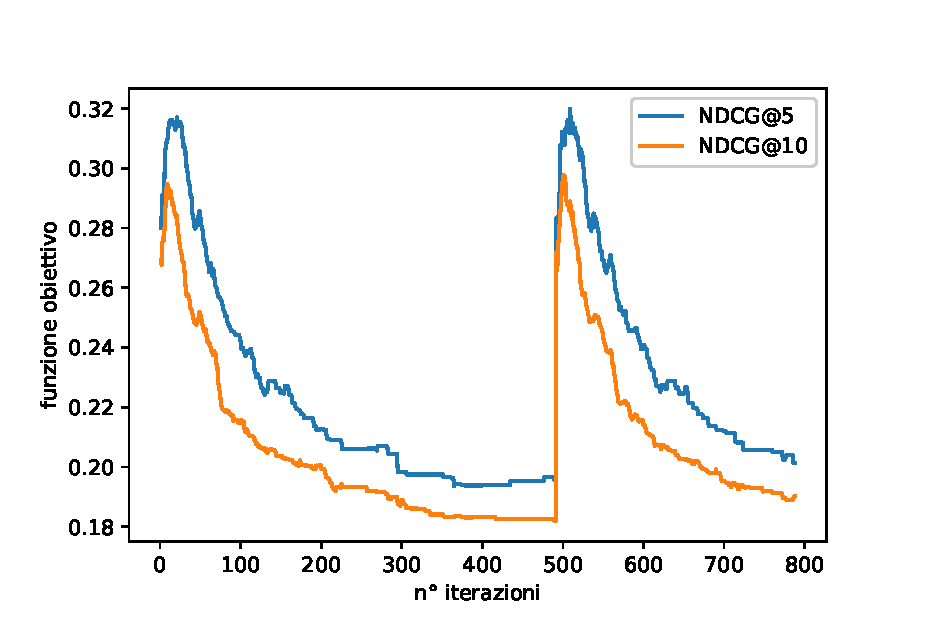
\includegraphics[width=0.7\linewidth]{figure/gs_search}
	\caption[Andamento della funzione obiettivo utilizzando GridSearch]{Andamento della funzione obiettivo in base al numero di iterazioni di GridSearch.}
	\label{fig:gssearch}
\end{figure}

La figura \ref{fig:gssearch} rappresenta il valore delle valutazioni in funzione del numero di iterazioni.

Si noti che il picco quando l'asse delle $x \approx 30$ corrisponde alla valutazione quando il vettore $w$ è variato
poco dal vettore iniziale.

\newpage

\section{Line Search with Random Restart}

Tale algoritmo è stato eseguito con gli stessi parametri di GridSearch e parallelizzato
su circa 16 processori differenti.

I risultati trovati sono i seguenti:

\begin{table}[h!]
	\centering
	\begin{tabular}{|c|c|c|c|}
		\hline
		\textbf{Misura} & \textbf{Valore} & \multicolumn{2}{|c|}{\textbf{Incremento} $\left[\%\right]$} \\
		\hline
		richiamo@100 &  0.1988 & $\downarrow$ & $-4.00$   \\
		\hline
		richiamo@200 & 0.2793  & $\downarrow$ & $-8.99$ \\
		\hline
		NDCG & 0.3814 & $\downarrow$ & $-8.33$\\
		\hline
		NDCG@5 & 0.3188 & $\uparrow$ & $+13.85$ \\
		\hline
		NDCG@10 & 0.2901 & $\uparrow$ & $+7.166$ \\
		\hline
		\multicolumn{4}{|c|}{
			$w = [1.071, 0.821, 0.821, 0.821, 0.821, 0.821, 1.071, 0.821, 1.0714, 1.071]$ 
		} \\
	\hline
	\end{tabular}
	\caption{Risultati di Line Search with Random Restart}
\end{table}

Anche questo algoritmo non porta a risultati soddisfacenti, principalmente  per il motivo
della grandezza di $\tau$ e della restrizione di $\mathcal{B}$.

\section{Increase Search}

L'ultimo risultato che verrà esposto è quello dell'algoritmo Increase Search, il quale
esito è più apprezzabile rispetto agli altri. Anche in questo caso l'esperimento
si è avvalso degli stessi parametri di configurazione e dello stesso budget temporale.

\begin{table}[h!]
	\centering
	\begin{tabular}{|c|c|c|c|}
		\hline
		\textbf{Misura} & \textbf{Valore} & \multicolumn{2}{|c|}{\textbf{Incremento} $\left[\%\right]$} \\
		\hline
		richiamo@100 &  0.1971 & $\downarrow$ & $-4.83$  \\
		\hline
		richiamo@200 & 0.2954 & $\downarrow$ & $-3.88$  \\
		\hline
		NDCG & 0.4119 & $\downarrow$ & $-1.01$ \\
		\hline
		NDCG@5 & 0.3542 & $\uparrow$ & $\mathbf{+26.5}$ \\
		\hline
		NDCG@10 & 0.3007 & $\uparrow$ & $\mathbf{+11.08}$ \\
		\hline
		\multicolumn{4}{|c|}{$w = [0.1981, 0.1012, 0.07532, 0.075321, 0.15023, 0.12532, 0.12512, 0.103, 0.0521, 0.2534]$} \\
		\hline
	\end{tabular}
	\caption{Risultati di Increase Search}
\end{table}

\pagebreak

\section{Risultati}

Com'è possibile notare il vettore dei pesi migliore è quello che è stato trovato
dall'algoritmo Increase Search, producendo un incremento del $26.5\%$ su NDCG@5
e del $11.08\%$ su NDCG@10, rispetto all'orginale BM25.

Pertanto, avendo a disposizione un budget di tempo $\mathcal{B}$ nell'ordine
delle ore, Increase Search è risultato il più performante rispetto agli altri.

Ovviamente aumentando $\mathcal{B}$ diventa possibile utilizzare altri
tipi di algoritmi, quali Grid Search o Line Search with Random Restart, che
forse potrebbero anche battere il record di Increase Search.

\section{Test di significatività statistico}

Prima di poter concludere che BM25P con il $w$ ottimo è migliore di BM25, è necessario
fare un test statistico, il cui obiettivo è quello di capire se $\text{BM25P}_w$ $\equiv$ BM25
cioè se essi sono uguali.

Il test di significatività statistica ha come scopo
quello di capire se due medie provengono da distribuzioni diverse oppure no.
Inannzitutto si deve formulare la \textit{null-hypothesis}, cioè l'ipotesi
della quale vogliamo provarne la falsità.

\begin{esempio}
	Si lancia un dado 10 volte e si calcola la media $\bar{X}_1$. Dopo un giorno si ripete l'esperimento
	e si ricalcola la media $\bar{X}_2$. Molto probabilmente si noterà che $\bar{X}_1 \neq \bar{X}_2$,
	ma tali valori provengono da distrubuzioni diverse?
	Ovviamente no, poiché i dadi sono gli stessi, dunque se la \textit{null-hypothesis} fosse
	stata $X_1 \equiv X_2$, allora avremmo potuto renderla vera.
\end{esempio}

Dunque in questo caso siamo in grado di accettare l'ipotesi perché
sapevamo già a priori che le due distribuzioni erano uguali, ma nel caso
in cui non lo sapessimo?
Uno dei modi più veloci di giudicare la \textit{null-hypothesis} è quello di eseguire un test statistico.
Accordandoci con l'articolo\cite{10.1145/1321440.1321528}, il migliore per valutare
due ranker è quello chiamato \textit{Fisher's Randomization Test}.

\subsection{Il test Randomizzato di Fisher}
Tale test si basa sull'ipotesi che due ranker $\mathcal{R}_1 $ e $\mathcal{R}_2$ siano identici
e che un altro ranker $\mathcal{R}_F$ si impossessi dei risultati di entrambi e
ritorni casualmente o quello di uno o quello di un altro.
Il ruolo giocato da $\mathcal{R}_F$ è di fondamentale importanza poiché esso produce un risultato
casuale tra i due; pertanto se essi fossero identici la distrubuzione non cambierebbe.
L'obiettivo principale però è quello di calcolare la probabilità che la differenza
di performance tra i due è soltanto dovuta al fatto che $\mathcal{R}_3$ sceglie casualmente
il risultato tra i due ranker.

Per eseguire il test ipotizziamo di avere a disposizione un dataset formato da una lista
di coppie $\langle e_{A}, e_{B}\rangle$, dove la lettera $e$ indica la funzione di valutazione
scelta: nel caso in questione NDCG@5. I pedici $A$ e $B$ indicano invece rispettivamente i due
ranker, dove per semplicità di trattazione abbiamo posto che $A$ è BM25P e $B$ è BM25. Tali valutazioni sono calcolate solo e soltanto su una query,
pertanto abbiamo a disposizione 50 coppie.

\paragraph{Definizioni}
Definiamo le seguenti quantità:

\begin{itemize}
	\item $N$ la lunghezza della lista del dataset (nel caso in questione $N=50$)
	\item $\sigma_A = \sum_{i=1}^{N} e_{A_i}$ e $\sigma_B = \sum_{i=1}^{N} e_{B_i}$
	\item $\bar{e}_A = \frac{\sigma_{A} }{N}$ e  $\bar{e}_B = \frac{\sigma_{B} }{N}$, cioè le relative medie aritmetiche
	\item $d = \sigma_{A} - \sigma_{B}$, cioè la differenza di performance tra i due ranker
\end{itemize}


\begin{algorithm}[h!]
	\SetAlgorithmName{Algoritmo}{}
	\small
	\DontPrintSemicolon
	\SetKwInOut{Input}{Input}
	\SetKwInOut{Output}{Output}
	\Input{$e_A$ lista delle valutazioni del ranker A}
	\Input{$e_B$ lista delle valutazioni del ranker B}
	\Input{$d$}
	\Input{$k$}
	\Input{$\sigma_A, \sigma_B$}
	\Input{$\bar{e}_A, \bar{e}_B$}
	\Output{$p_1,p_2$}
	\BlankLine
	$p_1 = 0, p_2 = 0$\;
	\BlankLine
	\For{$i=1$ \textbf{to} $k$}{
		$a,b = \text{randomChoice}(e_A, e_B)$\;
		$\bar{a} = avg(a)$\;
		$\bar{b} = avg(b)$\;
		
		\BlankLine
		$\delta = \bar{a} - \bar{b}$\;
		\If{$\delta \geq d$}{
			$p_1 = p_1 + 1$\;
		}
		\If{$\left|\delta\right| \geq \left|d\right|$}{
			$p_2 = p_2 + 1$\;
		}
	}
	
	\Return{$\frac{p_1}{k}, \frac{p_2}{k}$}
	\label{alg:spectest}
	\caption{Algoritmo per l'esecuzione del test di randomizzazione di Fisher}
\end{algorithm}

A questo punto si procede scegliendo un numero massimo $k$ di permutazioni
da eseguire poichè  senza limitazioni  il test avrebbe complessità $\mathcal{O}(2^N)$
e dunque per valori di $N$ elevati ci vorrebbe troppo tempo per eseguirlo.
\\
\\
Successivamente l'algoritmo esegue un ciclo, scorrendo un indice fino ad arrivare a $k$.
Nel corpo del ciclo, esso prende a caso un elemento della lista di $e_A$ o di $e_B$ e
calcola la differenza di qualità ottenuta.
A seconda dei risultati vengono incrementati i valori $p_1$ o $p_2$, che costituiscono
l'output dell'algoritmo stesso.

Riassumendo, ciò che $\mathcal{R}_3$ esegue è un assegnamento casuale di etichette e
possiamo considerare il test valido se la scelta è casuale (anche se in questo caso
dobbiamo accontentarci della pseudocasualità).

\paragraph{Il risultato del test}
I valori calcolati dall'algoritmo, cioè $p_1$ e $p_2$, sono due rapporti:

\begin{itemize}
	\item $p_1$ è detto anche ``one-sided-p-value", ovvero il rapporto tra il numero di volte in cui la differenza
	della valutazione è più grande di quella ipotizzata e il numero di permutazioni;
	\item $p_2$ è detto invece ``two-sided-p-value", ovvero il solito significato di $p_1$, ma utilizzando
	come metrica di differenza il valore assoluto.
\end{itemize}


Per poter valutare dunque la veridicità della \textit{null-hypothesis} si usano tali valori,
cioè $p_1$ e $p_2$ costituiscono un'approssimazione della probabilità che i due ranker
siano uguali. Solitamente si sceglie un valore $\alpha < 0.05$ per cui si valuta che
se $p_1$ e $p_2$ sono maggiori di $\alpha$ allora l'ipotesi non può essere rifiutata,
mentre se sono minori l'ipotesi è falsa e dunque i due ranker sono diversi.

\pagebreak

\subsection{Esecuzione nel caso di BM25P}
L'esperimento è stato condotto sul solito dataset, isolando le query dal\textit{ topic file} e calcolando NDCG
per ogni ogni query, sia con BM25 che con BM25P.

Il test ha riportato i seguenti valori:

\begin{table}[h!]
	\centering
	\begin{tabular}{|c|c|c|}
		\hline
		\textbf{Misura} & $p_1$ & $p_2$ \\
		\hline
		NDCG  & 0.13218 & 0.26347 \\
		\hline
		NDCG@5 & 0.00082 & 0.00145 \\
		\hline
		NDCG@10 & 0.03454 & 0.06835 \\
		\hline
	\end{tabular}
	\caption{Risultati del test statistico su BM25P}
\end{table}

Considerando i valori standard di $\alpha$, la \textit{null-hypothesis} (BM25P $\equiv$ BM25) può essere considerata falsa.
Questo perché, dato che l'ottimizzazione di BM25P è stata basata su tagli più piccoli, il test di significatività statistico su NDCG@5 e NDCG@10 
deve avere più peso rispetto a NDCG senza tagli.
Questo risultato inoltre ci mostra che i due ranker, su tagli più grandi, potrebbero essere simili, in quanto $p_2 > p_1 > \alpha$.

All'interno dell'appendice è stato inserito anche una parte di codice in Python che implementa
l'algoritmo.
